\chapter{Equilibrium $\beta$-limits of canonical configurations}

\section{Rotating ellipse}

\subsection{Ideal equilibrium $\beta$-limit in a classical stellarator} \label{sec.idealbetalimit}

In this section, it is shown that the \ac{SPEC} current constraint can be used to recover the \ac{HBS} theory prediction of the classical stellarator ideal equilibrium $\beta$-limit \citep{Freidberg2014,wakatani_stellarator_1998}, when zero net toroidal current is considered.  

A previous study \citep{Loizu2017} showed remarkable agreement between \ac{SPEC} calculations and the \ac{HBS} theory in a simplified case, with the pressure profile approximated by a single step. An additional limitation, enforced by the \ac{SPEC} version at that time, was that the vacuum region had to be approximated by a large plasma volume where the pressure and currents were set to zero, and a fixed-boundary would be applied. This approach is equivalent to assuming a free-boundary calculation with an infinitely conducting wall at the computational boundary. At large $\beta$, however, a strong Shafranov shift is present, and this approximation could have an impact on the result.

To understand the effect of these assumptions we consider here both fixed- and free-boundary calculations with a stepped-pressure profile approximating a Solov'ev's profile $p = p_0(1-\psi_t / \psi_a)$ where $\psi_a$ is the total toroidal flux enclosed by the plasma. The computational boundary is defined by Eqs.(\ref{eq.RotEllipse_R})-(\ref{eq.RotEllipse_Z}). Fixed-boundary calculations were made first, with seven plasma volumes surrounded by an eighth large, vacuum-like volume so that it is similar to a free-boundary calculation. The toroidal flux profile has been chosen such that $\psi_a=\sum_{l=1}^7\psi_{t,l}=0.25\text{Tm}^2$ and $\psi_{t,8} = 0.75\text{Tm}^2$, leading to a total toroidal flux enclosed by the plasma and the vacuum-like region of $\sum_{l=1}^8\psi_{t,l} = 1\text{Tm}^2$. Free-boundary input files were generated to replicate the same equilibrium in vacuum, using $\mu_0I_{coil}=21.43$Tm and $\psi_a=0.25\text{Tm}^2$, which correspond to an equilibrium with $\psi_{t,V}=0.75\text{Tm}^2$. In both fixed- and free-boundary calculations, both the surface currents and the volume currents were set to zero, \textit{i.e.} $I_{\phi,l}^{vol} = I_{\phi,l}^{surf} = 0$ for all $l$. The only control parameter remaining is $p_0$, which was increased in order to increase the plasma average $\beta$ until a central $m=1,\ n=0$ island opens. The island emerges when the rotational transform at the plasma edge, $\iotabar_a$, \textit{i.e.} the rotational transform on the outer side of the plasma-vacuum interface, reaches zero (see Figure \ref{fig:poincare}). This is defined as the ideal equilibrium $\beta$-limit. 

The physical mechanisms leading to the emergence of a separatrix are complex. In brief, the combination of non-zero poloidal harmonics of the Pfirsch-Schlüter and diamagnetic currents at the volumes' interfaces and the effect of the Shafranov shift perturbs sufficiently the poloidal magnetic field so that the rotational transform at the plasma edge decreases, until eventually it reaches zero. These results will be explained in more detail in a future publication.


The \ac{HBS} theory, building on the pioneering work of Greene and Johnson's stellarator expansion theory \citep{greene_determination_1961}, predicts that

\begin{equation}
	\iotabar_a = (\iotabar_v + \iotabar_I)(1-\nu^2)^{1/2},\label{eq.HBS_1}
\end{equation}
with $\iotabar_v$ the rotational transform at the plasma edge in vacuum and $\iotabar_I$ a contribution from the plasma toroidal current,

\begin{equation}
	\iotabar_I = \frac{\mu_0I_\phi R_{00}}{2\pi a^2B_0},
\end{equation}
with $I_\phi$ the total toroidal plasma current, $B_0$ the magnetic field strength on axis and $a$ the effective minor radius at the plasma edge, \textit{i.e.} $a=\sqrt{\psi_a / (\psi_a + \psi_{t,V})} r_{eff}$, with $r_{eff}$ the effective radius of the ellipse, given by the square root of the product between the ellipse major radius $r_{max}=|R_{10}+R_{11}|$ and the ellipse minor radius $r_{min}=|Z_{10}+Z_{11}|$, \textit{i.e.} $r_{eff}=\sqrt{r_{max}r_{min}}$. The parameter $\nu$ is defined as

\begin{equation}
	\nu = \frac{\langle\beta\rangle}{\epsilon_a(\iotabar_v+\iotabar_I)^2},
\end{equation}
with $\langle\beta\rangle$ the volume averaged plasma $\beta$ and $\epsilon_a = a / R_{00}$. Setting $\iotabar_a=0$ in Eq.(\ref{eq.HBS_1}) and solving for $\langle\beta\rangle$ leads to a prediction for the ideal equilibrium $\beta$-limit,

\begin{equation}
	\langle\beta\rangle_{lim,HBS} = \epsilon_a(\iotabar_v+\iotabar_I)^2.
\end{equation}
In the case of interest, $R_{00}=10$m, $R_{10}=-Z_{10}=1$m, $R_{11}=Z_{11}=0.25$m, leading to $r_{eff}\approx0.97$m and $a\approx0.48$m. Using $I_\phi=0$A, and $\iotabar_v\approx0.28$, one obtains $\langle\beta\rangle_{lim,HBS}\approx0.38\%$.

\begin{figure}
	\centering
	\hfill
	\subfloat[][$\langle\beta\rangle = 0\%$, $\iotabar_a\approx0.28$]{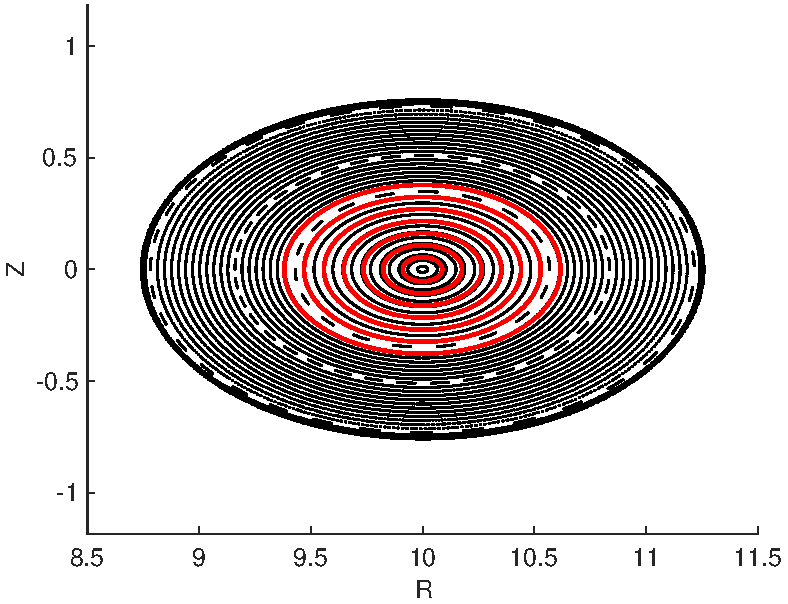
\includegraphics[width=0.3\linewidth]{main/Figures_CurrentConstraint/ABaillod_fig11a.pdf}}
	\hfill
	\subfloat[][$\langle\beta\rangle \approx 0.31\%$, $\iotabar_a\approx0.13$]{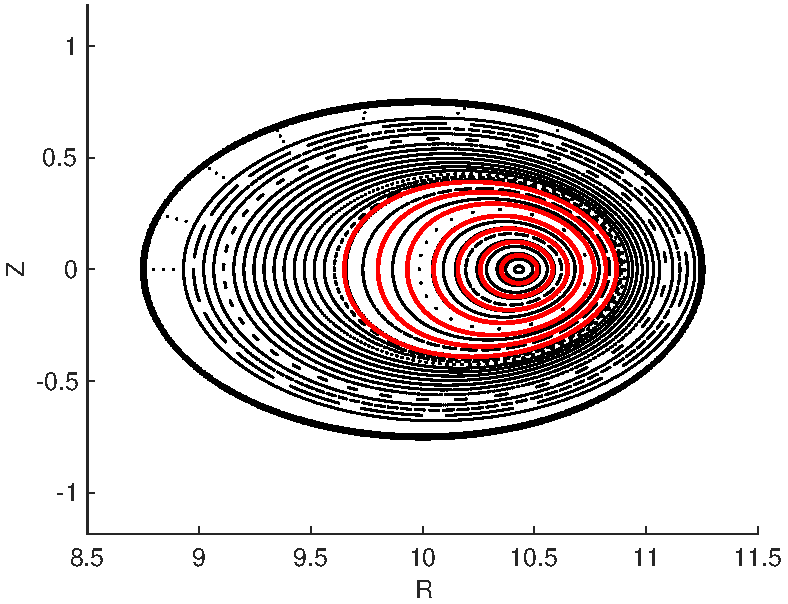
\includegraphics[width=0.3\linewidth]{main/Figures_CurrentConstraint/ABaillod_fig11b.pdf}}
	\hfill
	\subfloat[][$\langle\beta\rangle \approx 0.62\%$, $\iotabar_a= 0.0$]{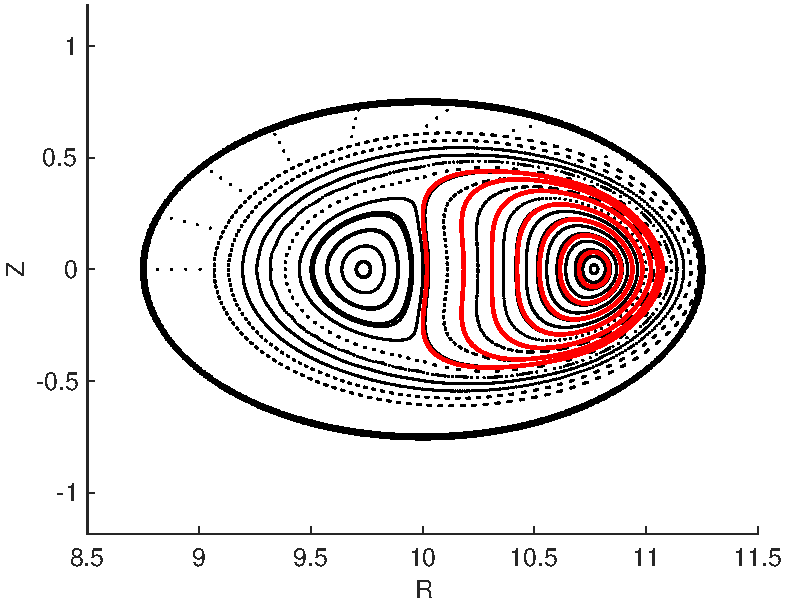
\includegraphics[width=0.3\linewidth]{main/Figures_CurrentConstraint/ABaillod_fig11c.pdf}}
	\hfill
	\caption{Poincar\'e plot of the magnetic field lines at $\phi=0$ and at three different values of $\langle\beta\rangle$ (a-c). Red surfaces are the volume interfaces and the black, bold surface is the computational boundary. In (c), the ideal equilibrium $\beta$-limit has been exceeded and a central island opened outside the plasma. A large value of $\langle\beta\rangle$ has been selected for illustration purposes.}
	\label{fig:poincare}
\end{figure}

Figure \ref{fig:iota_beta_scan} shows the rotational transform profile at different values of $\langle\beta\rangle$ (left) and the values of $\iotabar_a$ obtained with \ac{SPEC} as a function of $\langle\beta\rangle$ and compares them to the analytical prediction given by Eq.(\ref{eq.HBS_1}) (right). Good agreement is observed between the fixed-boundary and free-boundary calculations, showing that the fixed-boundary assumption made by \citet{Loizu2017} has only a small effect on the ideal equilibrium $\beta$-limit prediction. In addition, the free-boundary calculation and the \ac{HBS} theory agree well, and predict approximately the same ideal equilibrium $\beta$-limit. The small but finite difference between the results is most likely due to the \ac{HBS} theory, which employs an expansion in aspect ratio $\epsilon$ and assumes that the plasma boundary is circular. In fact, the number of volumes used in \ac{SPEC} to approximate the continuous pressure profile does not significantly influence the result of this study (data not shown).

\begin{figure}
	\centering
	\hfill
	\subfloat[][]{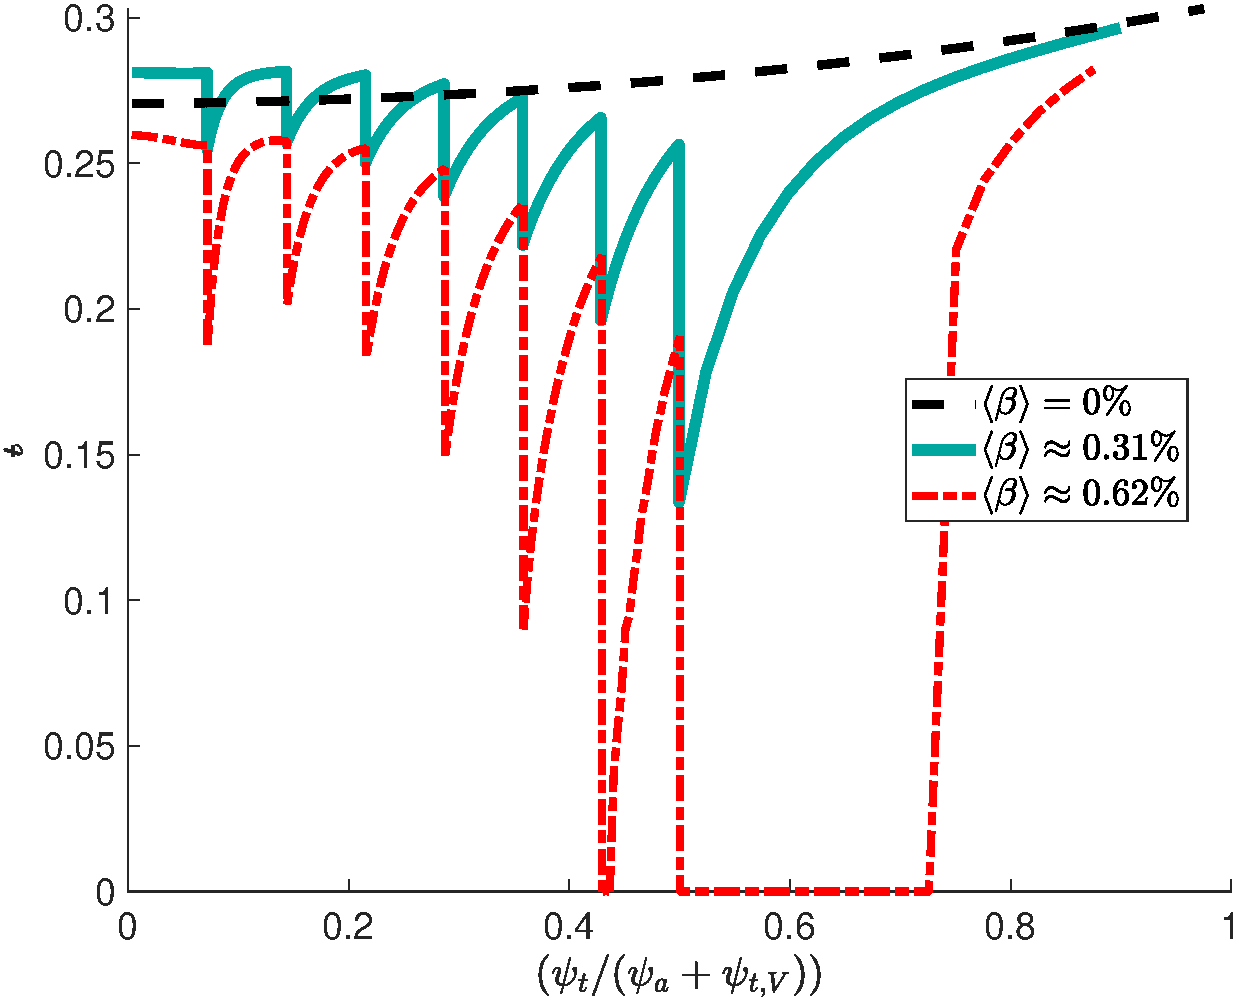
\includegraphics[width=0.45\textwidth]{main/Figures_CurrentConstraint/ABaillod_fig12a.pdf}}
	\hfill
	\subfloat[][]{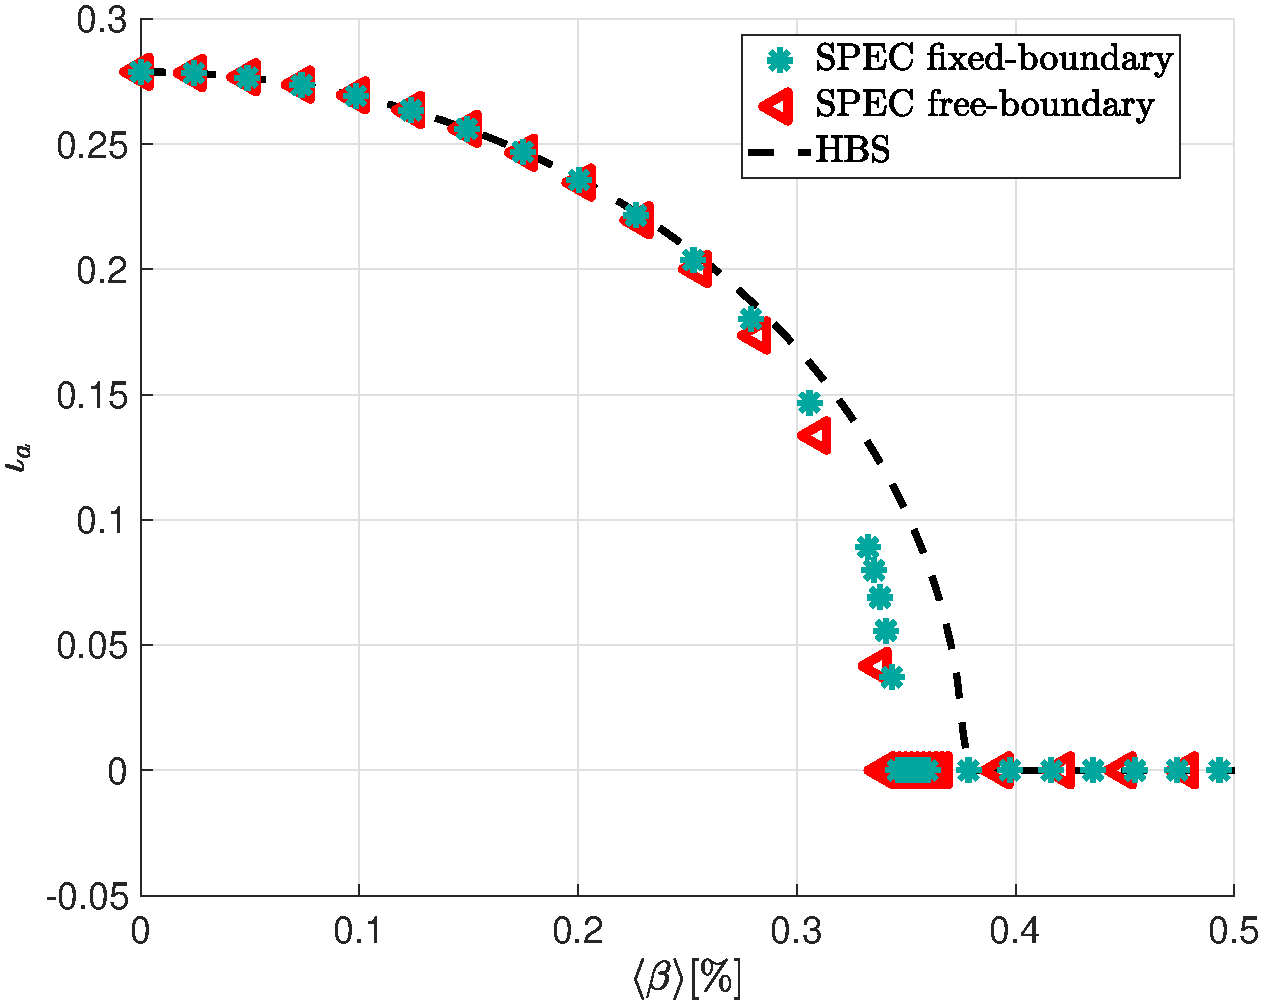
\includegraphics[width=0.45\textwidth]{main/Figures_CurrentConstraint/ABaillod_fig12b.pdf}}
	\hfill
	\caption{Left: rotational transform profile at three different values of $\langle\beta\rangle$, for free-boundary calculation of a rotating ellipse with zero net toroidal current. Right: rotational transform at the plasma edge as a function of $\langle\beta\rangle$. Comparison between free-, fixed-boundary and the \ac{HBS} theory.}
	\label{fig:iota_beta_scan}
\end{figure}


As a final remark, note that in our calculations, the plasma boundary is topologically constrained to be an ideal surface and cannot undergo re-connection. Another important constraint is that the pressure profile is fixed and cannot evolve. Other approaches without these constraints could lead to different results and conclusions. One natural question is then to ask about the physical validity of constraining the topology of a set of flux surfaces in \ac{MRxMHD}. First studies about the existence of \ac{MRxMHD} interfaces have been carried out \citep{McGann2010,Qu2021}, pointing towards certain existence criteria. The present study, however, aims at verifying the implementation of the toroidal current constraint in \ac{SPEC} by retrieving well established mathematical results. Future work will focus on code validation by using experimental data.



\section{QA}

\section{QH}

\section{QI}